% Appendix Template

\chapter{Definiciones Matemáticas} % Main appendix title

\label{AppendixB} % Change X to a consecutive letter; for referencing this appendix elsewhere, use \ref{AppendixX}

\lhead{Appendix B. \emph{Definiciones Matemáticas}} % Change X to a consecutive letter; this is for the header on each page - perhaps a shortened title

\section{Propiedades de las Matrices}

A continuación se muestran las definiciones básicas de las matrices que serán utilizadas para las simulaciones.

\subsection{Dependencia e independencia lineal}

Dado un conjunto finito de vectores $\mathbf{v}_1, \mathbf{v}_2,\cdots, \mathbf{v}_n$, se dice que dichos vectores son linealmente
independientes si existen números $a_1$, $a_2$, $\cdots$, $a_n$, donde la ecuación
$$
 a_1 \mathbf{v}_1 + a_2 \mathbf{v}_2 + \cdots + a_n \mathbf{v}_n = \mathbf{0} 
$$
se satisface únicamente cuando $a_1, a_2,\cdots, a_n$ son todos cero. En caso contrario, se dice que son linealmente dependientes.

Nótese que el símbolo a la derecha del signo igual no es cero, sino que simboliza al vector nulo $\mathbf{0}$. El conjunto de
vectores nulos forma la matriz nula. Si tales números no existen, entonces los vectores son linealmente independientes. La 
definición anterior también puede extenderse a un conjunto infinito de vectores, concretamente un conjunto cualquiera de 
vectores es linealmente dependiente si contiene un conjunto finito que sea linealmente dependiente.

Utilizando conceptos de espacios vectoriales se puede redefinir la independencia lineal de la siguiente forma:

Un conjunto de vectores $\textbf{U}$ de un espacio vectorial es linealmente independiente si 
$\forall u \in U, u \notin \langle U - u \rangle$

Esta idea es importante dado que los conjuntos de vectores que son linealmente independientes generan un espacio vectorial y 
forman una base para dicho espacio. Entre las propiedades de los vectores linealmente dependientes e independientes se pueden 
listar:
\begin{enumerate}
   \item Un conjunto de vectores es linealmente dependiente si y solamente si alguno de los vectores es combinación lineal de 
        los demás.
    \item Si un conjunto de vectores es linealmente independiente cualquier subconjunto suyo también lo es.
    \item Si un conjunto de vectores es linealmente dependiente, también lo es todo conjunto que lo contenga.
    \item Un conjunto de vectores son linealmente dependientes si y sólo si son paralelos.
    \item Un conjunto de vectores son linealmente dependientes si los componentes entre ellos son proporcionales, bien sea 
        directa o inversamente proporcional. Ya que un conjunto de vectores es linealmente dependiente si y solo si tiene algún
        vector que es combinación lineal de los demás \cite{MatrixDep}.
\end{enumerate}

\subsection{Rango de una matriz}

En álgebra lineal, el rango de una matriz es el número máximo de columnas (filas respectivamente) que son linealmente 
independientes. El rango fila y el rango columna siempre son iguales: este número es llamado simplemente rango de A.
Comúnmente se expresa como $rg(A)$ \cite{MatrixRg}.

El número de columnas independientes de una matriz $A$ de $m$ filas y $n$ columnas es igual a la dimensión del espacio columna
de $A$. También la dimensión del espacio fila determina el rango. El rango de A será, por tanto, un número no negativo, menor
o igual que el mínimo entre m y n:

\begin{equation}
    A \in M_{mxn} \Rightarrow 0 \le rg(A) \le min(m, n)
\end{equation}

\subsection{Determinate de una Matriz}

Para una matriz cuadrada $\mathbf{A}[n,n]$, el determinante de $\mathbf{A}$, abreviado $det(\mathbf{A})$, es un escalar definido
como la suma de $n!$ términos involucrando el producto de $n$ elementos de la matriz, cada uno proveniente exactamente de una 
fila y columna diferente. Además, cada término de la suma está multiplicado por $-1$ ó $+1$ dependiendo del número de 
permutaciones del orden de las columnas que contenga.

\subsubsection{Propiedades}

A continuación se listan las propiedades del determinante de las matrices cuadradas.
\begin{enumerate}
    \item $det(\mathbf{AB}) = det(\mathbf{A})det(\mathbf{B})$. Nota: esta propiedad vale solo si \textbf{A} y \textbf{B} son 
        matrices cuadradas.
    \item $det(\mathbf{A}^T) = det(\mathbf{A})$.
    \item $det(\mathbf{A}^H) = conj(det(\mathbf{A}))$, en donde $\mathbf{A}^H$ es la transpuesta conjugada (Hermítica) de \textbf{A}.
    \item $det(c\mathbf{A}) = cn\cdot det(\mathbf{A})$.
    \item Intercambiando cualquier par de columnas (filas) de una matriz se multiplica su determinante por $-1$.
    \item Multiplicando cualquier columna (fila) de una matriz por $c$ multiplica su determinante por $c$.
    \item Agregando cualquier múltiplo de una columna (fila) de una matriz a otra no altera su determinante.
    \item $det(\mathbf{A}) <> 0$ si y sólo si \textbf{A} no es singular, en otras palabras si es una matriz invertible \cite{MatrixDet}.
\end{enumerate}

\section{Cuadrados mínimos} \label{sec:meanSquare}
Esta sección describe una estrategia de resolución para cuando un problema, del tipo $\mathbf{Ax} = \mathbf{b}$, no tienen solución. 
La solución encontrada devuelve una \textbf{x} que deje a \textbf{Ax} tan cercana a \textbf{b} como sea posible.  

Si \textbf{A} es de $m x n$ y \textbf{b} está en $\mathds{R}^m$, una solución por mínimos cuadrados de $\mathbf{Ax} = \mathbf{b}$
es una $\hat{x}$ en $\mathds{R}^n$ tal que

$$
\parallel \mathbf{b} - \mathbf{A\hat{x}}\parallel \le \parallel\mathbf{b}-\mathbf{Ax} \parallel
$$

para toda \textbf{x} en $\mathds{R}^n$.

El aspecto más importante del problema de mínimos cuadrados es que no importa cuál \textbf{x} se elija, el vector \textbf{Ax}
necesariamente estará en el espacio de columnas. Así que se busca un \textbf{x} adecuado para convertir a \textbf{Ax} en el 
punto de Col \textbf{A} más cercano a \textbf{b}. (Por supuesto, si sucede que \textbf{b} está en Col \textbf{A}, entonces 
\textbf{b} es \textbf{Ax} para algún \textbf{x}, y tal \textbf{x} es una “solución por mínimos cuadrados”.)

El conjunto de soluciones por mínimos cuadrados de $\mathbf{Ax} = \mathbf{b}$ coincide con el conjunto no vacío de soluciones
de las ecuaciones normales $\mathbf{A}^T\mathbf{Ax} = \mathbf{A}^T\mathbf{b}$ \cite{MatrixMin}.

\section{Matriz Hadamard}
Esta matriz fue descubierta por el matemático Jacques Hadamard, es una matriz cuadrada con valores $1$ o $-1$ y sus columnas 
son ortogonales. Sus propiedades son las siguientes \cite{HadamardWiki}. 

Si se tiene una matriz $H$ de orden $n$, su traspuesta está cercamente relacionada con su inversa. Y su fórmula es:

$$ H H^{\mathrm{T}} = n I_n $$

Donde $I_n$ es la matriz de identidad de dimensión $n x n$ y $H^\mathrm{T}$ es la traspuesta de $H$. Esta propiedad es válida a causa 
que las columnas de $H$ son vectores ortogonales en el campo de los números reales y cada uno tiene una longitud de $\sqrt n$.
Dividiendo H por su longitud, se obtiene una matriz ortonormal que su traspuesta también es su inversa. El determinante es:

$$ \operatorname{det}(H) = \pm n^{\frac{n}{2}} $$

Donde $\operatorname{det}(H)$ es el determinante de $H$.

Si se supone que $M$ es una matriz compleja de orden n, con valores que cumplen la relación $|M_{ij}| \le 1$, por cada $i,j$ 
entre 1 y $n$. Entonces el determinante de la matriz hadamard resulta,
		    
$$ |\operatorname{det}(M)| \leq n^{n/2}. $$

La igualdad es válida solamente si $M$ es real y solo si $M$ también es una matriz Hadamard.

El orden de una matriz hadamard debe ser 1, 2 o un múltiplo de 4.

\subsection{Construcción de Silvester}

Los primeros ejemplos de construcción de matrices Hadamard fueron realizados por James Joseph Sylvester en 1867. Si H es 
dicha matriz de orden $n$, su construcción es como sigue.

$$ \begin{bmatrix} H & H\\H & -H\end{bmatrix} $$

Resulta una matriz de Hadamard de orden $2n$. Este proceso puede ser repetido para obtener las matrices siguientes, 
conocidas también como matrices Walsh. 

$$ H_1 = \begin{bmatrix} 1 \end{bmatrix}, $$

$$  H_2 = \begin{bmatrix} 1 & 1 \\ 1 & -1 \end{bmatrix}, $$

and

$$ H_{2^k} = \begin{bmatrix} H_{2^{k-1}} & H_{2^{k-1}}\\ H_{2^{k-1}} & -H_{2^{k-1}}\end{bmatrix} $$

para $2 \le k \in N$.


\section{Parámetros S} \label{sc:appendixSParam}

La sigla S deriva de la palabra dispersión. Para altas frecuencias, es conveniente describir una
determinada red en términos de ondas en vez de tensiones o corrientes. Esto permite una definición más
sencilla de planos de referencia. Por razones prácticas, la descripción en términos de ondas entrantes
y salientes ha sido introducida. Ahora, una red de 4 polos se transforma en 2 puertos y $2n$ polos se
transforman en $n$ puertos. En el caso de un número impar de polos (ej. 3 polos), un punto de referencia
puede ser elegido, atribuyendo un polo igualmente a dos puertos. Por lo tanto 3 polos se convierten en
3 + 1 polo correspidiendo a 2 puertos. Como una regla general, para cantidades impares de polos, siempre
se agrega un polo extra.

\begin{figure}[H]
 \centering
 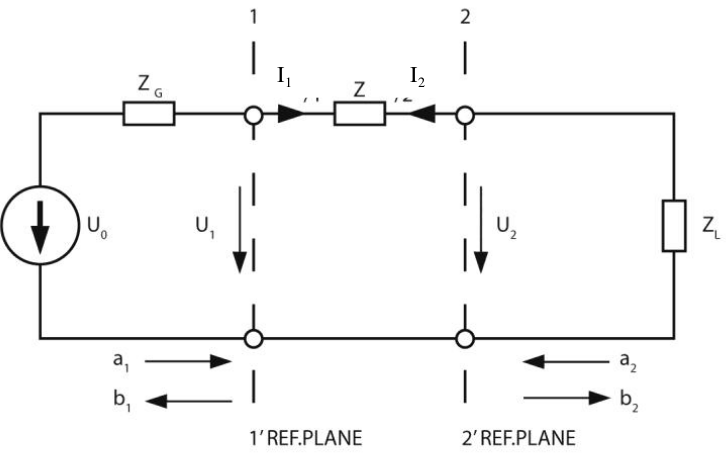
\includegraphics[width=10cm]{gfx/sParameters1.png}
 \caption{Ejemplo de una red de 2 puertos: circuito serie}
 \label{fig:esquema_serie}
\end{figure}

Tomando como ejemplo una red de 2 puertos compuesta por una sola impedancia $Z$ conectada en serie (\ref{fig:esquema_serie}).
Las impedancias de la fuente y de la carga son $Z_G$ y $Z_L$ respectivamente. Si $Z=0$ y $Z_L = Z_G$ (para el caso de $Z_G$ real)
la carga está adaptada. En este caso se obtiene una máxima transferencia de potencia y $U_1 = U_2 = U_0/2$. Notar que todas las
tensiones y corrientes son valores pico. Se supone que las líneas que unen los componentes poseen longitud eléctrica igual a 0.
Las conecciones con una longitud eléctrica finita están dibujadas como una doble líea. A continuación se relacionará $U_0$, $U_1$
y $U_2$ a $a$ y $b$.


\subsection{Definición de \enquote*{ondas de potencia}}

Las ondas incidentes al puerto son $\textbf{a}=(a_1, a_2, a_3, ..., a_n)$, las ondas salientes, o reflejadas, del puerto son
$\textbf{b}=(b_1, b_2, b_3, ..., b_n)$. Por definición, las corrientes incidentes son positivas y las salientes negativas. La
onda $a_1$, incidente al puerto 1, es derivada de la tensión entrante a la carga balanceada.

Para hacer qe esta definición sea consistente con la ley de la conservación de la energía. La tensión es normalizada a $\sqrt{Z_0}$.
$Z_0$ es, en general una impedancia de referencia arbitraria, que usualmente se la utiliza como la impedancia característica de la
línea (ej, $Z_0 = 50 \Omega$). Y, cuando todas las impedancias son iguales ($Z_G = Z_L = Z_0$), se dice que la línea está adaptada
y no hay onda reflejada. Las definiciones de $a1$ y $b1$ son:

\begin{equation}
\begin{aligned}
	a1 &= \dfrac{U_0}{2\sqrt{Z_0}}= \dfrac{\textrm{onda de tensión incidente (puerto 1)}}{\sqrt{Z_0}}=\dfrac{U_1^{inc}}{\sqrt{Z_0}} \\
	b1 &= \dfrac{U_1^{refl}}{2\sqrt{Z_0}}= \dfrac{\textrm{onda de tensión reflejada (puerto 1)}}{\sqrt{Z_0}}
\end{aligned}
\end{equation}

Notar que \textbf{a} y \textbf{b} tienen las unidades de $\sqrt{\textrm{potencia}}$.

La potencia incidente al puerto 1, $P_{inc}$, es simplemente la potencia entregada por la fuente, mientras que la potencia saliente
del puerto 1, $P_{refl}$, viene de la onda de tensión reflejada.

\begin{equation}
\begin{aligned}
	P_1^{inc} &= \dfrac{1}{2}|a_1|^2= \dfrac{|U_1^{inc}|^2}{2Z_0}=\dfrac{|I_1^{inc}|^2}{2}Z_0 \\
	P_1^{refl} &= \dfrac{1}{2}|b_1|^2= \dfrac{|U_1^{refl}|^2}{2Z_0}=\dfrac{|I_1^{refl}|^2}{2}Z_0 \\
\end{aligned}
\end{equation}

En el caso de una desadaptación de la impedancia de carga $Z_L$, parte de la potencia será reflejada a través del puerto 2 (
potencia incidente al puerto 2).

$$
P_2^{inc}=\dfrac{1}{2}|a_2|^2
$$

Se ha definido $a_1 = U_0/2\sqrt{Z_0} = U^{inc}/\sqrt{Z_0}$ con la onda de tensión incidente $U^{inc}$. Como analogía
se la puede definir como $a_1 = I^{inc}\sqrt{Z_0}$ con la onda incidente de corriente $I^{inc}$. Utilizando ambas, se obtiene la
definición general de las ondas incidentes $a_i$ y reflejadas $b_i$ de un puerto.

\begin{equation}
\begin{aligned}
	a_i &= \dfrac{U_i + I_iZ_0}{2\sqrt{Z_0}} \\
	b_i &= \dfrac{U_i - I_iZ_0}{2\sqrt{Z_0}}
\end{aligned}
\label{eq:waves}
\end{equation}

Solucionando este sistema de ecuaciones, $U_i$ y $I_i$ pueden ser obtenidas de $a_i$ y $b_i$ como

\begin{equation}
\begin{aligned}
	U_i &= \sqrt{Z_0}(a_i + b_i) = U_i^{inc} + U_i^{refl}\\
	I_i &= \dfrac{1}{\sqrt{Z_0}}(a_i - b_i) = \dfrac{U_i^{refl}}{Z_0}
\end{aligned}
\end{equation}


\subsection{La matríz de parámetros S}

La relación entre $a_i$ y $b_i$ (siendo $i=1..n$) puede ser escrito como un sistema de n ecuaciones lineales (siendo la variable
independiente $a_i$ y $b_i$ como la dependiente)

\begin{equation}
\begin{aligned}
	b_1 = S_{11}a_1 + S_{12}a_2 \\
	b_2 = S_{21}a_1 + S_{22}a_2
\end{aligned}
\label{eq:s_matrix}
\end{equation}

Escrito de forma matricial: \textbf{b} = \textbf{Sa}

El significado físico de los parámetros S son los siguientes:
\begin{itemize}
	\item $S_{11}$: es el coeficiente de reflexión con la salida de la red terminada en una carga adaptada ($a_2 = 0$).
	\item $S_{21}$: es la transmisión en directa (del puerto 1 al 2)
	\item $S_{12}$: es la transmisión en inversa (del puerto 2 al 1)
	\item $S_{22}$: es el coeficiente de reflexión de la salida.
\end{itemize}

Al medir todos los parámetros S de una red de n puertos, todos los puertos deben estar terminados con una carga adaptada.
Utilizando las equaciones \ref{eq:waves} y \ref{eq:s_matrix} se obtiene el coeficiente de reflexión de una impedancia $Z_L$
conectada a un generador de impedancia de salida $Z_0$ (Figura \ref{fig:esquema_serie}, caso $Z_G = Z_0$ y $Z = 0$):

\begin{equation}
S_{11} = \dfrac{b_1}{a_1}\bigg|_{a_2=0} = \dfrac{U_1 - I_1Z_0}{U_1 + I_1Z_0} = \dfrac{Z_L - Z_0}{Z_L + Z_0} = \Gamma
\end{equation}


\subsection{La matriz de transferencia} \label{ssec:transMatrix}

Resulta muy conveiente la utilización de la matriz de parámetros S para describir una red de n polos en términos de ondas y
para mediciones. Pero, no es muy conveniente su utilización para caracterizar la respuesta de una cascada de redes de 2
puertos. En este caso, una manera de encarar dicha problemática, es la utilización de la matriz de parámetros T (matriz
de transferencia), la cual relaciona las ondas de entrada y salida de cada cuadripolo.

\begin{equation}
\begin{pmatrix} a_1\\b_1 \end{pmatrix} = \begin{pmatrix} T_{11} & T_{12}\\T_{21} & T_{22} \end{pmatrix}
\begin{pmatrix} a_2\\b_2 \end{pmatrix}
\end{equation}

Cabe destacar que, para los casos en que no hay transmisión entre el puerto 1 y 2, si bien la matriz de parámetros S está definida,
la matriz de parámetros T no. La matriz resultante de parámetros T de una cascada de redes de 2 puertos resulta como sigue:

\begin{equation}
\mathbf{T_M=T_1T_2...T_m}
\label{eq:cascade}
\end{equation}

\subsection{Conversión entre parámetros T y S} \label{ssec:conversion}

Como la matriz de transferencia (T) simplemente relaciona las ondas de entrada y salidas de una forma diferente a la matriz de
scattering, partiendo de una matriz se puede llegar a la otra y viceversa.

\begin{equation}
	\begin{aligned}
		T_{11} &= S_{12} - \dfrac{S_{22}S_{11}}{S_{21}},\quad T_{12} = \dfrac{S_{11}}{S_{21}} \\
		T_{21} &= - \dfrac{S_{22}}{S_{21}},\qquad\qquad T_{22} = \dfrac{1}{S_{21}}
	\end{aligned}
	\label{eq:s2t}
\end{equation}

Para obtener los parámetros S partiendo desde los parámetros T, se utiliza la siguiente relación matemática

\begin{equation}
	\begin{aligned}
		S_{11} &= \dfrac{T_{12}}{T_{22}},\qquad S_{12} = T_{11} - \dfrac{T_{12}T_{21}}{T_{22}} \\
		S_{21} &= \dfrac{1}{T_{22}},\qquad S_{22} = - \dfrac{T_{21}}{T_{22}}
	\end{aligned}
	\label{eq:t2s}
\end{equation}


\subsection{Propiedades de la matriz de parámetros S}

Una red generalizada de n puertos posee $n^2$ coeficientes de scattering. Mientras que los $S_{ij}$ podrían ser todos independientes,
en general, debido a simetrías u otros factores, la cantidad de coeficientes independientes es mucho menor.
\begin{itemize}
	\item Una red de n puertos es recíproca cuando $S_{ij} = S_{ji}$ para todo $i, j$. La mayoría de los componentes pasivos son
		recíprocos (resistencias, capacitores, transformadores, etc., exceptuando para estructuras involucrando ferrites magnéticos,
		plasmas, etc.), componentes activos como amplificadores generalmente son no recíprocos.
	\item Una red de 2 puertos es simétrica cuando es recíproca ($S_{21} = S_{12}$) y cuando los coeficientes de reflexión son iguales
		($S_{11} = S_{22}$).
	\item Una red de N puertos es pasiva y sin pérdidas si su matriz de parámetros S es unitaria ($\mathbf{S^{\dagger}S = 1}$ donde
		$\mathbf{x^{\dagger} = (x^*)^T}$ es la conjugada y transpuesta de $x$). Para una red de 2 puertos esto significa

\begin{equation}
S^{\dagger}S = \begin{pmatrix} S_{11}^* & S_{21}^*\\S_{12}^* & S_{22}^* \end{pmatrix}
			\begin{pmatrix} S_{11} & S_{12}\\S_{21} & S_{22} \end{pmatrix} = \begin{pmatrix} 1 & 0\\0 & 1 \end{pmatrix}
\end{equation}

Esto conlleva a 3 condiciones

\begin{equation}
\begin{aligned}
	|S_{11}|^2 + |S_{21}|^2 = 1 \\
	|S_{12}|^2 + |S_{22}|^2 = 1 \\
	S_{11}^*S_{12} + S_{21}^*S_{22} = 0
\end{aligned}
\label{eq:sCondition}
\end{equation}

Separando la última ecuación en módulo y fase, se obtiene

\begin{equation}
\begin{aligned}
	|S_{11}||S_{12}| &= |S_{21}||S_{22}| \\
	-argS_{11} + argS_{12} &= -argS_{21} + argS_{22} + \pi
\end{aligned}
\label{eq:con}
\end{equation}

Donde $arg(x)$ es el argumento (angulo) de la variable compleja $x$. Combinando la ecuación \ref{eq:sCondition} con la primera
de la ecuación \ref{eq:con} se obtiene

\begin{equation}
\begin{aligned}
	|S_{11}| = |S_{12}|, |S_{21}| = |S_{22}| \\
	|S_{11}| = \sqrt{1 - |S_{12}|^2}
\end{aligned}
\end{equation}

Por lo tanto, cualquier red de 2 puertos sin pérdidas puede ser caracterizada con un módulo y tres ángulos.
\end{itemize}

En general los parámetros S son valores complejos y dependientes de la frecuencia.
